\section{System development II: Quantification of microbial structures}

ImageJ, like most image processing software packages, is well-equipped to conduct the image pre-processing described in the previous section. However, for the quantification of binary representations of filamentous microbes, additional functionality was required. This section provides a description of the plug-ins that were developed to this end, together with a summary of the complete analysis procedure for fungal spores and hyphal elements at the microscopic level and, on the macroscopic scale, fungal pellets. All routines described in this study were written in Java, incorporating ImageJ classes and methods where appropriate.

\subsection{Microscopic analysis}\label{sec:MicroAnalysis}

While image pre-processing is similar regardless of the object of interest, the analysis of hyphal elements is more extensive than that of spores. The steps involved in each case are presented (Fig.~\ref{fig:MicroAlg}). It is assumed that a colour (RGB colour-space) image is provided as input, but this is not strictly necessary.

\begin{figure}[htbp]
	\centering
	\pstool[width=12cm]{../C2/MicroAlg}{
		\psfrag{S}[Bc]{\al\hspace{2mm}Start}
		\psfrag{F}[Bc]{\al\hspace{2mm}Filter}
		\psfrag{R}[Bc]{\al\hspace{2mm}Obtain Red Channel}
		\psfrag{T}[Bc]{\al\hspace{2mm}Threshold}
		\psfrag{I}[Bc]{\al\hspace{2mm}Isolate}
		\psfrag{i}[Bc]{\al\hspace{2mm}Objects}
		\psfrag{s}[Bc]{\al\hspace{2mm}Spores}
		\psfrag{h}[Bc]{\al\hspace{2mm}Hyphae}
		\psfrag{k}[Bc]{\al\hspace{2mm}\emph{Skeletonise}}
		\psfrag{B}[Bc]{\al\hspace{2mm}Binary \emph{Close}}
		\psfrag{W}[Bc]{\al\hspace{2mm}\emph{Watershed}}
		\psfrag{P}[Bc]{\al\hspace{2mm}\emph{Prune}}
		\psfrag{A}[Bc]{\al\hspace{2mm}Analyse Hyphae}
		\psfrag{Y}[Bc]{\al\hspace{2mm}Yes}
		\psfrag{N}[Bc]{\al\hspace{2mm}No}
		\psfrag{f}[Bc]{\al\hspace{2mm}Finish}
		\psfrag{O}[Bc]{\al\hspace{2mm}Open Next Image}
		\psfrag{r}[Bc]{\al\hspace{2mm}Analyse Spores}
		\psfrag{L}[Bc]{\al\hspace{2mm}Last}
		\psfrag{l}[Bc]{\al\hspace{2mm}Image?}}
	\caption{Algorithm used for characterization of fungal micro-morphology}
	\label{fig:MicroAlg}
\end{figure}

The image is divided into three, 8-bit grey-scale images, representing the three primary colour components (red, green and blue). The red component exhibits the greatest contrast for images of lactophenol cotton blue-stained samples (a common mycological preparation) and is retained for image processing; the green and blue components are discarded. Image pre-processing begins with filtering of the image to compensate for low-frequency, uneven illumination using an implementation of the Rolling Ball algorithm \cite{sternberg1983}. The radius of the filter was set to the pixel equivalent of \mic{40} (40 pixels for images of hyphae, 200 pixels for spores), which is large relative to the width of a typical hypha (approximately \mic{2 -- 4}). Any high-frequency speckle noise was subsequently removed by median filtering. A grey-level threshold, calculated using the iso-data algorithm was then applied, resulting in a binary image.

The next stage of the routine is dependent on whether spores or hyphae are the primary object of study. It is unlikely that viable spores and hyphae will be present in the same image: results from this study indicated that the majority of spores had germinated by approximately 8~hours after inoculation (data not shown). Any spores present in a sample taken after this time were considered to be non-viable and were treated by the system as artifacts.

\subsubsection{Analysis of spores}

In the case of spores,  a \emph{watershed} operation was used to separate any touching objects. Objects were then classified based on projected area and circularity\footnote{In the case of a circle, $\Ap=\pi r^2$ and $P=2\pi r$, and so $C=1$. The larger $P$ becomes with respect to $\Ap$, the less circular the object becomes and so the value of $C$ decreases}. Spores of many industrially relevant fungi, such as \emph{Aspergillus}, are relatively spherical \cite{spohr1998}. Therefore, objects with a projected area above a specified minimum ($\Apm$) and with a circularity greater than a threshold value ($\Csm$) were considered to be spores; remaining objects were considered to be artifacts and were excluded from the analysis.

\subsubsection{Analysis of mycelia}

When hyphae are the objects of interest, a single binary \emph{close} operation (a single \emph{dilation} operation followed by a single \emph{erosion}) is performed to remove any small breaks (or holes) in the objects. All objects with a projected area below $\Apm$ or a circularity greater than a second threshold value ($\Chm$) are excluded from the analysis. The binary image of the hyphal elements is then \emph{skeletonised}, which reduces the objects in the image to a series of lines one pixel in width.

The \emph{skeletonisation} of an object during image analysis can occasionally result in artifactual points or branches \cite{packer1990,drouin1997,spohr1998}. Artifactual points (sites where the skeleton is greater than one pixel in width) can lead to the incorrect classification of branch-points, while artifactual branches can lead to an over-estimation of hyphal length and the number of hyphal tips. These may be removed by way of \emph{pruning} (Fig.~\ref{fig:PruneAlg}), which also has the effect of removing any remaining small artifacts from the image. 

\begin{figure}[htbp]
	\centering
	\pstool[width=(\textwidth - 1cm)]{../C2/PruneAlg}{
		\psfrag{S}[Bc]{\al\hspace{2mm}Start}
		\psfrag{s}[Bc]{\al\hspace{2mm}Scan Image}	
		\psfrag{Y}[Bc]{\al\hspace{2mm}Yes}
		\psfrag{N}[Bc]{\al\hspace{2mm}No}
		\psfrag{F}[Bc]{\al\hspace{2mm}Finish}
		\psfrag{A}[Bc]{\al\hspace{2mm}Artifactual}
		\psfrag{a}[Bc]{\al\hspace{2mm}Point?}
		\psfrag{R}[Bc]{\al\hspace{2mm}Remove}
		\psfrag{E}[Bc]{\al\hspace{2mm}End of}
		\psfrag{e}[Bc]{\al\hspace{2mm}Image?}
		\psfrag{T}[Bc]{\al\hspace{2mm}Tip?}
		\psfrag{t}[Bc]{\al\hspace{2mm}Trace Element}
		\psfrag{O}[Bc]{\al\hspace{2mm}Tip or}
		\psfrag{o}[Bc]{\al\hspace{2mm}Branch-point?}
		\psfrag{B}[Bc]{\al\hspace{2mm}Branch-length}
		\psfrag{b}[Bc]{\al\hspace{2mm}$>$ Minimum?}}
	\caption{Algorithm used for the \emph{pruning} of skeletal hyphal structures prior to measurement}
	\label{fig:PruneAlg}
\end{figure}

The \emph{pruning} routine begins by scanning the image in a raster fashion until a black pixel is located. If this pixel is deemed artifactual (by way of a look-up table), then it is removed. This process continues until the end of the image has been reached. The second stage begins by scanning the image in a raster fashion until a hyphal tip is located. A tip is defined as a black pixel with just one other black pixel in the immediate neighbourhood (Fig.~\ref{fig:ClassPoints}). The location of the tip is recorded and the skeleton is then traced from this tip along the hyphal length until either another tip or branch-point is reached. A branch-point is defined as a black pixel with three or more black pixels in the immediate neighbourhood, with no two of these neighbours joined. The length of the branch is then calculated based on the number of pixels traversed. If the length of the branch is less than the specified minimum ($\Lbm$) it is removed. The scan of the image then resumes from the point where the initial tip was located and the process continues until the end of the image has been reached. All pre-processing of mycelia is illustrated in Figure~\ref{fig:MyceliaProc}.

\begin{figure}[tb]
	\centering
	\subfloat[]{\label{fig:ClassPointsa}
\includegraphics[width=4cm]{../C2/ClassPointsa}}
	\hspace{1cm}
	\subfloat[]{\label{fig:ClassPointsb}
\includegraphics[width=4cm]{../C2/ClassPointsb}}
	\\
	\subfloat[]{\label{fig:ClassPointsc}
\includegraphics[width=4cm]{../C2/ClassPointsc}}
	\hspace{1cm}
  \subfloat[]{\label{fig:ClassPointsd}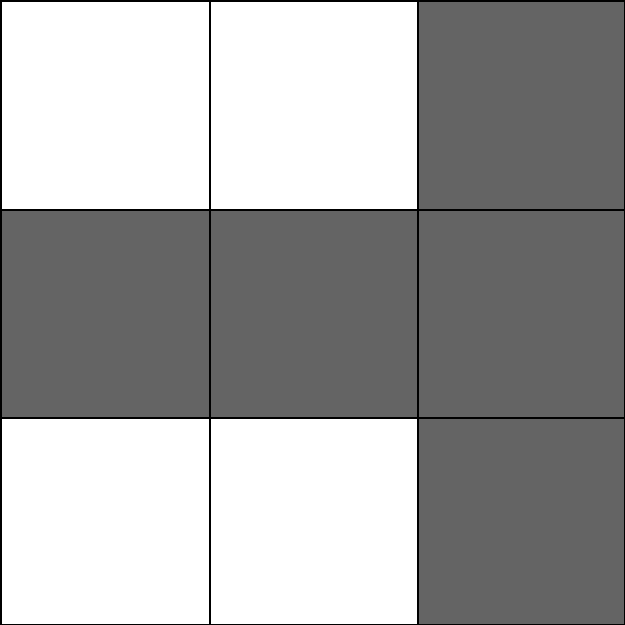
\includegraphics[width=4cm]{../C2/ClassPointsd}}
  \caption{Classification of points on a skeletal hyphal structure. (a) A pixel is defined as a hyphal tip if all but one of the neighbouring pixels is white. (b) If two of the neighbouring pixels are black, the current pixel is deemed an internal component of a hyphal \emph{segment}. (c) A branch-point is defined if at least three neighbouring pixels that do not share a common edge are black. (d) Conjoined neighbouring black pixels indicate the current pixel is adjacent to a branch-point}
  \label{fig:ClassPoints}
\end{figure}

\begin{figure}[tb]
	\centering
	\subfloat[]{\label{fig:MyceliaProca}\fbox{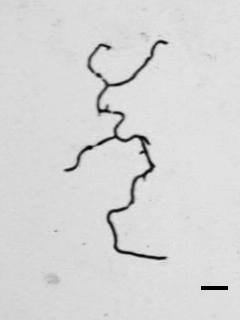
\includegraphics[width=3.1cm]{../C2/MyceliaProca}}}
	\hspace{0.2cm}
	\subfloat[]{\label{fig:MyceliaProcb}\fbox{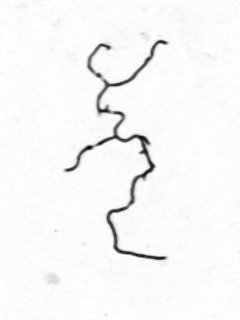
\includegraphics[width=3.1cm]{../C2/MyceliaProcb}}}
	\hspace{0.2cm}
	\subfloat[]{\label{fig:MyceliaProcc}\fbox{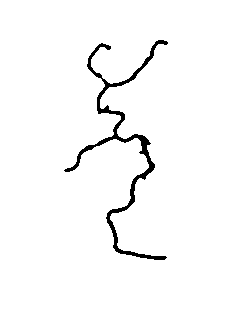
\includegraphics[width=3.1cm]{../C2/MyceliaProcc}}}
	\hspace{0.2cm}
  \subfloat[]{\label{fig:MyceliaProcd}\fbox{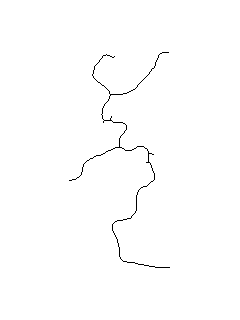
\includegraphics[width=3.1cm]{../C2/MyceliaProcd}}}
  \caption{(a) Original image of stained mycelium produced using the protocols described in Sections~\ref{sec:OptAssay} \& \ref{sec:microscopy} (Bar \mic{30}) (b) Background subtracted and median filtered (c) Resultant binary image (d) \emph{Pruned}, \emph{skeletonised} mycelium.}
  \label{fig:MyceliaProc}
\end{figure}

Once \emph{pruned}, the \emph{skeletonised} hyphae are suitable for analysis (Fig.~\ref{fig:HAAlg}). The routine begins by scanning the image in a raster fashion until a hyphal tip is located. The location of the tip is noted and the skeleton is then traced from this tip along the hyphal length until either another tip or branch-point (collectively termed \emph{end-points}) is reached. At this point, the length of the branch is recorded, along with the position and classification of the end-points. This combined information describes a hyphal \emph{segment}. For example, unbranched hyphae will consist of a single \emph{segment} with two tips as \emph{end-points}.

\begin{figure}[htbp]
	\centering
	\pstool[width=(\textwidth - 1cm)]{../C2/HyphalAnalyseAlg}{
		\psfrag{S}[Bc]{\al\hspace{2mm}Start}
		\psfrag{s}[Bc]{\al\hspace{2mm}Scan Image}	
		\psfrag{Y}[Bc]{\al\hspace{2mm}Yes}
		\psfrag{N}[Bc]{\al\hspace{2mm}No}
		\psfrag{E}[Bc]{\al\hspace{2mm}End of}
		\psfrag{e}[Bc]{\al\hspace{2mm}Image?}
		\psfrag{T}[Bc]{\al\hspace{2mm}Tip?}
		\psfrag{t}[Bc]{\al\hspace{2mm}Trace Element}
		\psfrag{O}[Bc]{\al\hspace{2mm}Tip or}
		\psfrag{o}[Bc]{\al\hspace{2mm}Branch-point?}
		\psfrag{r}[Bc]{\al\hspace{2mm}Output Results}
		\psfrag{R}[Bc]{\al\hspace{2mm}Store Result}
		\psfrag{C}[Bc]{\al\hspace{2mm}Element}
		\psfrag{c}[Bc]{\al\hspace{2mm}Complete?}}
	\caption{Algorithm used for the analysis of skeletal hyphal elements}
	\label{fig:HAAlg}
\end{figure}

If a branch-point is located, tracing continues along the first \emph{segment} found branching away from this point; any additional \emph{segments} branching from this point are \emph{pushed} onto a \emph{stack}, containing \emph{segments} yet to be traced. If a hyphal tip is reached, the current \emph{segment} is recorded and the most recently encountered, non-traced \emph{segment} is \emph{popped} from the top of the \emph{stack}, and the routine continues tracing from there.

If a tip is reached and all \emph{segments} in the current hyphal element have been traced, the measured data (total hyphal length, number of tips, and hyphal growth unit) is outputted to the results table. The algorithm then returns to the point in the image where the last hyphal element was first located and continues to scan until either another element is detected or the end of the image is reached.

\subsubsection{Generation of Mycelium Graph}

The compiled information on the individual \emph{segments} of a mycelial structure may be thought of as a mycelium graph or network (Fig.~\ref{fig:MyceliumGraph}). Each tip and branch-point represent the vertices of the graph, connected by edges whose length is that of the hyphal \emph{segment} from which it was derived.  Such a representation of a mycelium is of use in calculating, for example, the length of the \lq main' hypha \cite{papagianni2006a}, or the distribution of tips or branch-points with respect to other branch-points. By fixing such a graph to a co-ordinate plane, it may also be used to geometrically map foraging strategies of the microbe.

\begin{figure}[t]
	\centering
	\fbox{
		\setlength{\unitlength}{1.59cm}
		\begin{picture}(3.77, 7.17)
			\put(0,0){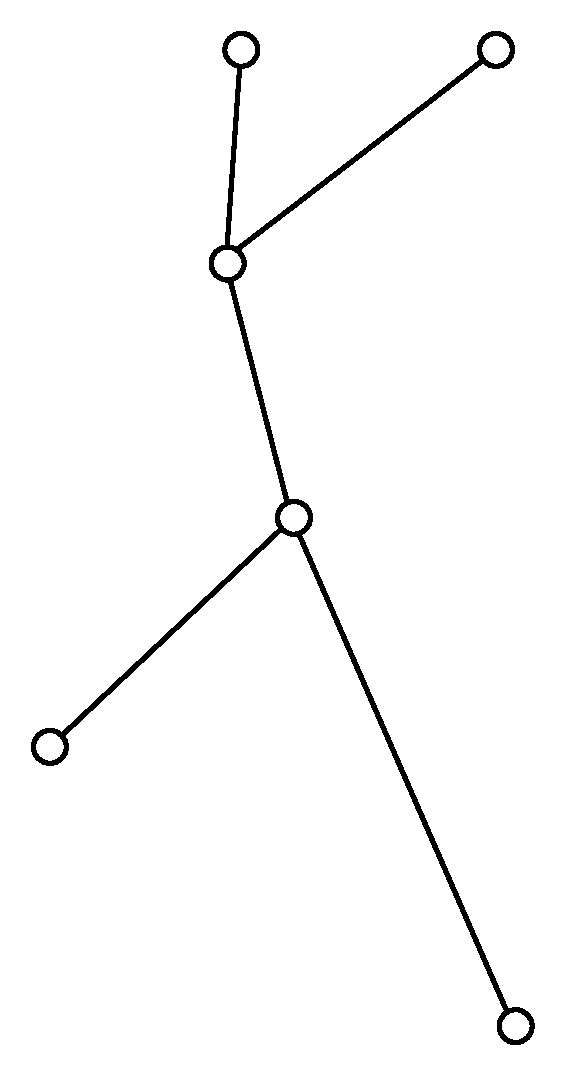
\includegraphics[width=5.99cm]{../C2/MycelialGraph}}
			\put(2.7,2.2){226.4}
			\put(0.6,3.0){64.6}
			\put(1.2,4.2){78.0}
			\put(1.0,6.2){58.1}
			\put(2.8,6.2){76.8}
		\end{picture}}
  \caption{Graph of the mycelium in Figure~\ref{fig:MyceliaProc} with small branches omitted for clarity.}
  \label{fig:MyceliumGraph}
\end{figure}

\subsubsection{Analysis of a population}

Typically, the morphological characterisation of a single hyphal structure is of limited value and with this in mind, the plug-ins described here have been adapted to process a series of images and derive population statistics. The programme begins by requesting a set of parameters from the user, along with the directory in which the bank of images to be analysed is contained. The routine then proceeds automatically until all images in the specified directory have been processed. An example of data output following the analysis of a population of mycelia is shown in Figure~\ref{fig:HGUResult}.

\begin{figure}[t]
	\centering
	\subfloat{\label{fig:HGUDist}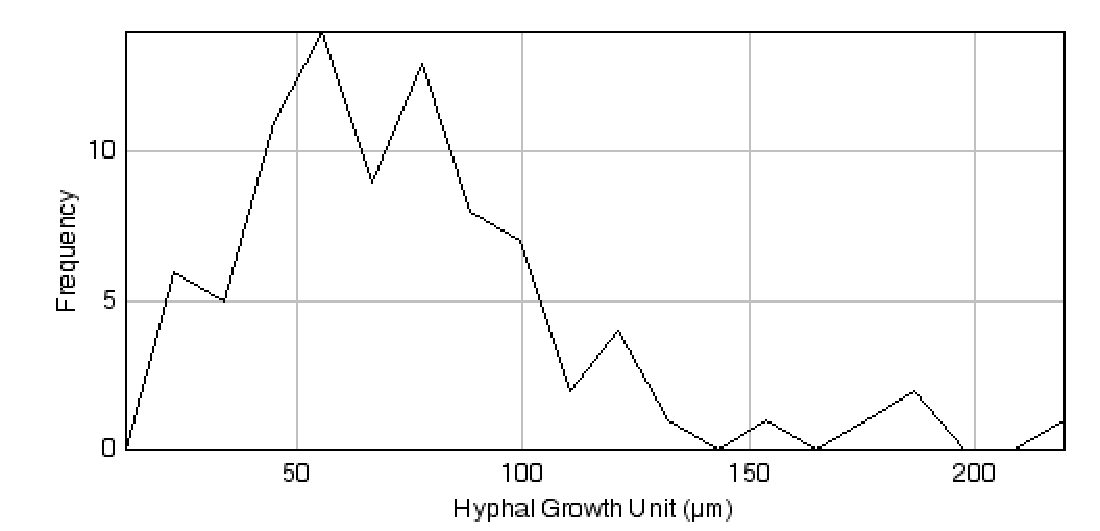
\includegraphics[width=10.5cm]{../C2/HGUDist}}
	\\
	\subfloat{\label{fig:HGUResults}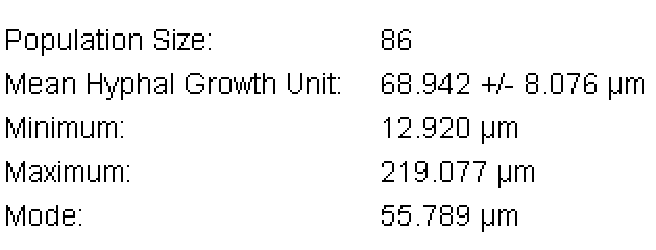
\includegraphics[width=8cm]{../C2/HGUResults}}
  \caption{Distribution and statistics on hyphal growth unit values produced in a typical analysis of a population of mycelial elements.}
  \label{fig:HGUResult}
\end{figure}

\subsection{Macroscopic analysis}\label{sec:MacroAnalysis}

Analysis of pellet images commences in a similar manner to that described above. The red channel of the RGB image is isolated and subject to the same filtering procedures as those used for microscopic images, albeit with a larger filter radius for background subtraction (8~mm). Prior to thresholding, it is necessary to locate the Petri dish in the image, so that a region-of-interest (ROI) may be specified within the Petri dish. This was achieved using a method similar to that described by D\"{o}rge and colleagues \cite{dorge2000}. To begin, a Sobel filter is applied to the image ($I$):

\begin{equation}
	\newcolumntype{L}{>{\raggedleft\arraybackslash}X}
		G_x = \left[ \begin{tabularx}{2.5cm}{L L L}
										1 & 2 & 1 \\
										0 & 0 & 0 \\
										-1 & -2 & -1
									\end{tabularx} \right] \ast I \mbox{\hspace{1cm}and\hspace{1cm}}
		G_y = \left[ \begin{tabularx}{2.5cm}{L L L}
										1 & 0 & -1 \\
										2 & 0 & -2 \\
										1 & 0 & -1
									\end{tabularx} \right] \ast I
\end{equation}

\noindent The resultant \lq edge image' is then Gaussian filtered to smooth and remove noise. The Petri dish may then be found by locating the nearest local maximum to a chosen image corner. This assumes that the Petri dish is approximately centrally located in the image. By repeating this operation for two more corners, three different points on the Petri dish circumference may be located, representing three points on a circle ($a$, $b$ and $c$). The centre of the circle ($o$) is then located by forming two chords ($ab$ and $ac$), bisecting them and calculating the point of intersection of the two perpendicular bisectors ($mo$ and $no$). A ROI, representing the Petri dish, may then be specified with $o$ as centre and $|oa|$ as the radius ($r$). However, considering the digital representation of the Petri dish is not perfectly circular (due to, for example, optical aberration), more accurate elimination is achieved if $r$ is specified as:

\begin{equation}
	r = (1 - T)|oa|
\end{equation}

\noindent where $T$ is some specified tolerance (typically 0.1). Once the ROI is specified, the region outside is cleared and the image may be thresholded as above. The entire process is illustrated in Figure~\ref{fig:PelletProc}. Quantification of objects in the resultant binary image is identical to that described above for spores. The morphological data corresponding to the image in Figure~\ref{fig:PelletProc} is shown in Figure~\ref{fig:PelletResult}.

\begin{figure}[tb]
	\centering
	\subfloat[]{\label{fig:PelletProca}\fbox{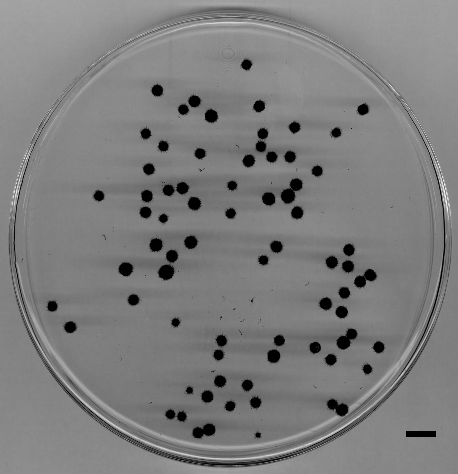
\includegraphics[width=4.2cm]{../C2/PelletProca}}}
	\hspace{0.3cm}
	\subfloat[]{\label{fig:PelletProcb}\fbox{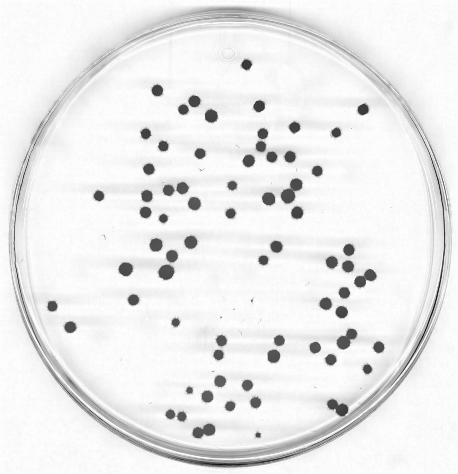
\includegraphics[width=4.2cm]{../C2/PelletProcb}}}
	\hspace{0.3cm}
	\subfloat[]{\label{fig:PelletProcc}\fbox{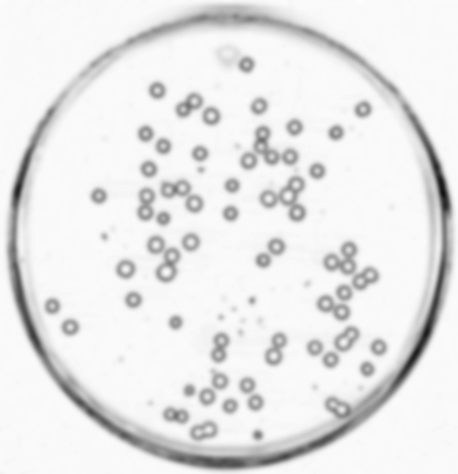
\includegraphics[width=4.2cm]{../C2/PelletProcc}}}
	\\
  \subfloat[]{\label{fig:PelletProcd}\fbox{\pstool[width=4.2cm]{../C2/PelletProcd}{
  	\psfrag{a}[Bc]{\al $a$}
		\psfrag{b}[Bc]{\al $b$}
		\psfrag{c}[Bc]{\al $c$}
		\psfrag{m}[Bc]{\al $m$}
		\psfrag{n}[Bc]{\al $n$}
		\psfrag{o}[Bc]{\al $o$}}}
	}
  \hspace{0.3cm}
  \subfloat[]{\label{fig:PelletProce}\fbox{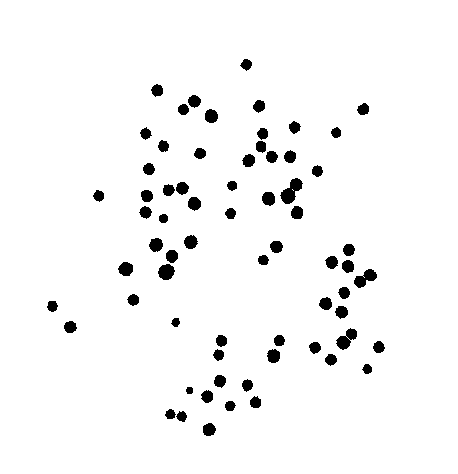
\includegraphics[width=4.2cm]{../C2/PelletProce}}}
  \caption{(a) Original image of stained pellets produced using the protocol described in Section~\ref{sec:PelletScan} (Bar 10~mm) (b) Background subtracted and median filtered (c) Gaussian filtered edge image (d) Points $a$, $b$ and $c$ are located on Petri dish circumference, midpoints $m$ and $n$ are found and $o$ is located as the intersection of the perpendicular bisectors of $ab$ and $ac$ (e) Resultant mask image.}
  \label{fig:PelletProc}
\end{figure}

\begin{figure}[htbp]
	\centering
	\subfloat{\label{fig:PelletDist}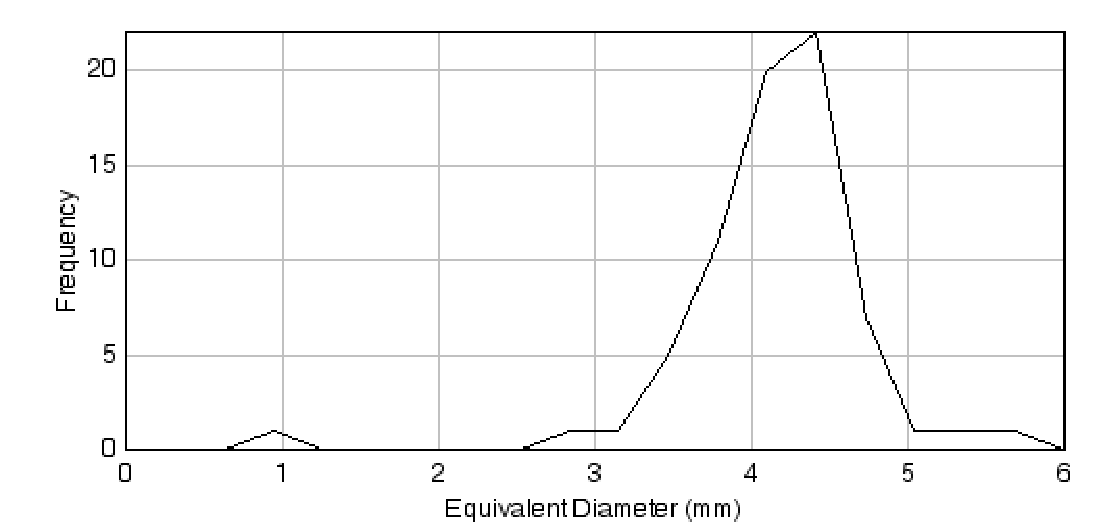
\includegraphics[width=10.5cm]{../C2/PelletDist}}
	\\
	\subfloat{\label{fig:PelletResults}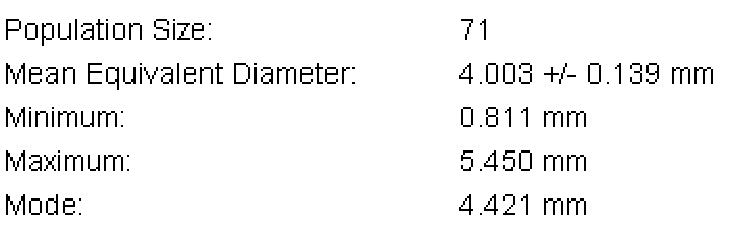
\includegraphics[width=8cm]{../C2/PelletResults}}
  \caption{Result of the analysis of the pellets in Figure~\ref{fig:PelletProc}.}
  \label{fig:PelletResult}
\end{figure}